
\subsection{MULTI-SCALE MATCH CRITERIA}
The match criteria to track object at images is based in the $PIV$ technique; 
where, a ROI and a Window Of Search ($WOS$) is defined; and is 
verified the similarity of $ROI$ over any part of $WOS$ using $PCC$. 
So that, the highest coefficient of Pearson determines the new location of the object.

Figure \ref{fig:multires}(a) shows a application in 2 dimensions, where
the $ROI$ information is searched, in the same scale,  in the entire image.

The Figure \ref{fig:multires}(b) reveals how the dimension of depth was included and
the search is made in different scales (layers); similarly to the $2D$ case, 
in 3 dimensions the target 
also is found through the highest $PCC$ among $WOS$, but the object found may be 
bigger or smaller, depending of in which layer the match happens. 
In all cases, before of be compared, the analyzed region in the $WOS$ was 
rescaled to have the same size that the $ROI$.

\begin{figure}[H]
\centering
  \subfloat[]{\label{subfig:(a)} 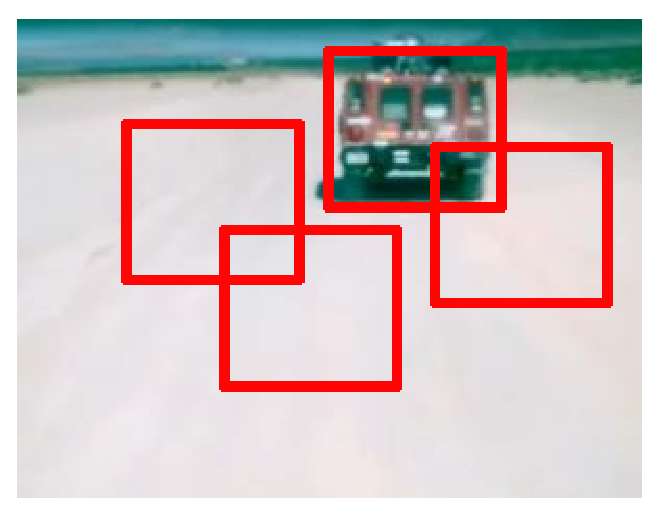
\includegraphics[width=.5\columnwidth]{images/figure2a.eps}}
  \subfloat[]{\label{subfig:(b)} 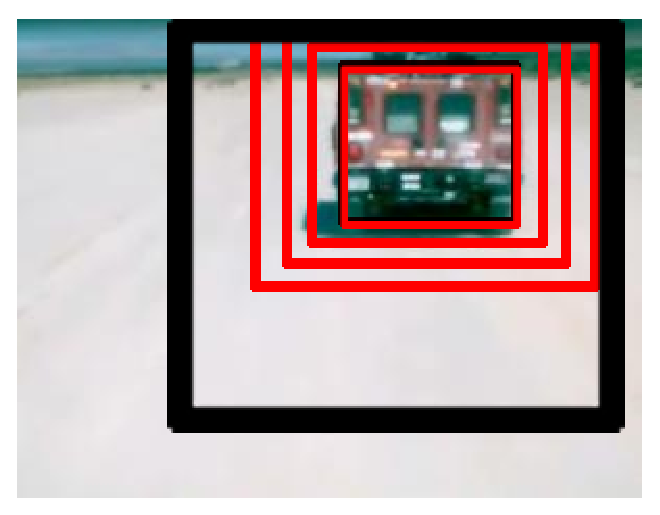
\includegraphics[width=.5\columnwidth]{images/figure2b.eps}}
  \caption{The red boxes show the analyzed regions and the black boxes represent the $WOS$. 
  (a) The regions are compared in the same scale with the $ROI$. 
  (b) The regions are compared with the $ROI$  using different scales.}
  \label{fig:multires}
\end{figure}




%onde estava, onde esta agora
%que tamanho tinha que tamanho tem.